\documentclass[english]{DESCARWINreport}
%pm[ForwardSearch("%bm.pdf","%Wc",%l,0,0,1)]
\usepackage{times}
\usepackage{helvet}
\usepackage{courier}
\usepackage{graphicx}
\usepackage{multirow}
%\usepackage[utf8]{inputenc}
\usepackage{algorithm}
\usepackage[noend]{algorithmic}
\usepackage{amsmath}
\usepackage{amsfonts}
\usepackage{amssymb}
\usepackage{array}
\usepackage{subfigure}
\usepackage{lscape}
%\usepackage{aaai}

\algsetup{indent=1.8em}
\renewcommand{\algorithmiccomment}[1]{// #1}
\newcommand{\pp}{planning tasks}
\newcommand{\PP}{planning task}
\newcommand{\dae}{{\em Divide-and-Evolve}}
\newcommand{\DAEI}{{\sc D\&E}}
\newcommand{\DAEII}{{\sc DaE2}}
\newcommand{\DAE}{{\sc DaE}}
\newcommand{\DAEX}{{\sc DaE$_{\text{X}}$}}
\newcommand{\DAEYAHSP}{{\sc DaE$_{\text{YAHSP}}$}}
\newcommand{\CPT}{{\sc CPT}}
\newcommand{\LPG}{{\sc LPG}}
\newcommand{\LAMA}{{\sc LAMA}}
\newcommand{\TFD}{{\sc TFD}}
\newcommand{\YAHSP}{{\sc YAHSP}}
\newcommand{\OPENSTACKS}{{\sc Openstacks}}
\newcommand{\ELEVATORS}{{\sc Elevators}}
\newcommand{\CREWPLANNING}{{\sc CrewPlanning}}
\newcommand{\FLOORTILE}{{\sc Floortile}}
\newcommand{\PARCPRINTER}{{\sc ParcPrinter}}

\def\modae{{\em Multiobjective Divide-and-Evolve}}
\def\MODAE{{\sc MO-DaE}}
\newcommand{\MODAEYAHSP}{{\sc MO-DaE$_{\text{YAHSP}}$}}
\newcommand{\MODAEX}{{\sc MO-DaE$_{\text{X}}$}}

\def\UU{{\mathbb{U}}}

%\title{DESCARWIN\\\bigskip {\em \LARGE The Marriage of Descartes and Darwin}\\\bigskip \bigskip \bigskip \bigskip \bigskip \bigskip \bigskip {\LARGE WP1: the \DAEX\ Planning System}}
%\title{DESCARWIN\\\bigskip {\em \LARGE The Marriage of Descartes and Darwin}\\\vspace{8cm} {\LARGE D6.2: Crisis Management Planning Benchmark}}
\title{DESCARWIN\\\bigskip {\em \LARGE The Marriage of Descartes and Darwin}\\
\vspace{8cm}
{\LARGE D6.2: Crisis Management Planning Benchmark}}
%\vfill
%
\includegraphics[width=.33\textwidth]{hd_logo_thales.jpg}
%
\includegraphics[width=.33\textwidth]{INRIA_logo.jpg}
%
\includegraphics[width=.33\textwidth]{ONERA_logo.jpg}}
%ANR-09-COSI-002
%\author{Pierre Sav�ant}
\date{\today}
\laboratory{TRT - INRIA - ONERA}
\docref{62 441 217-179-6}

\revision{-}


%\setlength{\parindent}{0cm}
%\setlength{\parskip}{2ex plus 0.5ex minus 0.2ex}


% Pour r�duire globalement l'espace entre les items d'une liste
% on peut �galement utiliser le bout de code suivant de M. Wooding
% Les param�tres utilis�s pour d�finir cette mise en page
% sont les suivants :
% \topsep espace vertical suppl�mentaire (ajoute � \parskip)
% 	ins�r� entre le texte pr�c�dant la liste et le 1er objet
% 	de la liste
% \partosep espace vertical suppl�mentaire ins�r� devant la liste
% 	si celle-ci est pr�c�d�e d'une ligne blanche
% \itemsep espace vertical suppl�mentaire (ajout� � \parsep)
% 	ins�r� entre les �l�ments d'une liste.

%%%% debut macro %%%%
\makeatletter
\toks@\expandafter{\@listI}
\edef\@listI{\the\toks@\setlength{\parsep}{0pt}}
\edef\@listI{\the\toks@\setlength{\topsep}{0pt}}
\makeatother
%%%% fin macro %%%%


\begin{document}

\maketitle

%\cleardoublepage

\begin{revisions}
\begin{revtable}
\dates{April 30, 2013}{}{}{}
\writers{Pierre Sav\'eant\\Florence Aligne}{}{}{}
\approvers{P. Sav\'eant}{}{}{}
\end{revtable}
\begin{revisionlabels}
\revlabel{initial version}
\revlabel{}
\end{revisionlabels}
\end{revisions}

\begin{abstract}
This document provides the description of the Crisis Management Benchmark which includes a generic set of actions (the domain) and a suite of grounded scenarios (or problems).
%This work has been partially presented at the 6th Future Security Conference in Berlin on Monday 5th September 2011.
The originality of the model is to take into account the impact of an urban traffic prediction on transit times thanks to the activity constraints presented in WP4.
We then designed a second domain in which a cost criterion is added, in order to provide a new benchmark to the multiobjective planner \MODAE\ developed in WP3.
\end{abstract}

\tableofcontents

\newpage

\chapter{Introduction}
A general assumption for offline planning is to consider that environmental changes are only caused by our own actions whereas in practice, it is obvious that 
there are other factors that affect how the environment evolves. Our aim is to take into account these exogenous evolutions, when they are predictable according to some forecast.
This capability is highlighted in the context of emergency and crisis management planning on an urban terrorist attack scenario where traffic congestion has a major impact on transit times.
The  traffic  evolution and  control  is  captured  with PDDL2.2  timed  initial
literals \cite{Edelkamp2004} which we implemented in the last release of the optimal temporal {\sc CPT} planner \cite{Vidal2006}.
Besides the crisis management rules and constraints, the model includes traffic evolution and control as well as dispatching casualties to hospitals. The emergency modeling is based on current operational protocols, whereas the traffic forecasting is based on statistical reference situations computed by an external traffic flow prediction module. Today, modern traffic forecasters, based on theoretical and empirical models, provide accurate short term forecasts suitable for good trip time estimates.

% State-of-the-art Crisis management at ICAPS
The main advantage in designing a crisis management planning domain in PDDL is first to produce a formal description of the domain and second to provide a great flexibility for changes. In \cite{Fdez-Olivares2006,Castillo2006} forest fighter fighting is addressed with the SIADEX Temporal HTN planner which extends HTN planning with Simple Temporal Networks, precedence and deadline constraints, and PDDL2.2 timed initial literals. Timed initial literals are used to forecast exogenous events but transportation times do not depend on the time they occur as we suggest to do. In \cite{Barbulescu2010a,Barbulescu2010b} the coordination of agents for a disaster response is handled with a multi-agent approach over a simple temporal network. The system is turned toward plan execution and repair whereas we are still in the design phase, at the beginning of the crisis, just before the dispatching of the casualties.

% Report outline
The remainder of the report is organized as follows. We first put up the crisis management context and emphasize on the need for a more global action coordination.
We then describe succinctly how modern traffic forecasters work. 
In the next section, we recall the constraint-based approach of CPT and give some clues on how timed initial literals are integrated in it.
We then present the PDDL emergency model with a focus on traffic evolution and control and the dispatching of casualties.
A multiobjectivization of the model is then introduced with the addition of a cost criteria in order to provide a multiobjective benchamark to \MODAE, the multiobjective release of \DAE\ described in WP3.
Finally, we discuss some generalizations and future challenges and conclude.

\chapter{Crisis Management Modeling}

Previous works have pointed out the lack of a global decision support system to coordinate the response to crises such as natural disasters, industrial accidents, or terrorist attacks \cite{Aligne2009,AligneSaveant2010}. Today, the response is structured and driven by a set of predefined protocols specific to the type of event, to the rescue team (e.g. police, firemen) and to the crisis extent (e.g. regional, local). Our aim is to integrate these protocols in a general model in order to synthesize emergency plans for a given crisis scenario with a planner.
For instance, the medical part of the rescue is a sequence of subtasks devoted to extraction, decontamination, triage and evacuation of casualties.
Rescue operations imply many actors such as the police, firemen and the medical services at least, but also, depending on the crisis type, road traffic services, railways companies, power suppliers, etc.. One of the main requirements is to improve the coordination of all the actors to get back to a normal situation (all casualties shall be evacuated, fires extinguished, etc.) as soon as possible. Therefore we retained in our model the total makespan as the main criterion.
The model is then refined with the task of routing casualties to the nearest hospitals, matching the type of casualties with hospitals having the required competencies.
This adds a capacity constraint to the model since hospitals have a bounded number of available beds for each type of injuries.

Since the metrics is time and the crisis zone an urban area, a close attention was given to transit times in the road network.
Due to the traffic flow, these transit times vary along the day with the time at which the trip occurs. Moreover police units have the possibility to alter the traffic by blocking roads.
This raises the question of forecasting the evolution of the crisis context and its integration in the planning task.

\chapter{Traffic Prediction Modeling}

Forecasting methods are generally based either on a statistical analysis, or on some predictable physical phenomenons. In traffic theory, statistical regression models have been developed such as the well known Bison Fut\'e in France based on SAS programming \cite{DanechPajouh2003}.
Alternatively, behavioral methods use either microscopic models in order to capture local interactions in urban traffic networks \cite{Treiber2000}, or macroscopic models considering road traffic as a fluid \cite{Haut2007,Lebacque2007}.

We collected statistical data provided by the French Direction Interd\'epartementale des Routes (DIR) on the Sytadin web site\footnote{www.sytadin.fr}. The data represent 456 km of rapid urban road, 331 km of national road with heavy traffic and 4 millions of vehicles per day. The traffic is usually monitored using three global indicators, the total length of jammed road (in km), the average speed value (in km/h), and a comparative congestion indicator (in \%). The analysis of one year data shows some daily trends in the volume of traffic, as shown on figure \ref{figure-traffic-repartition-by-day} \cite{SytadinDayHourRepartition2004}.

\begin{figure}[h!]
\begin{center}
%\vskip -0.3cm
%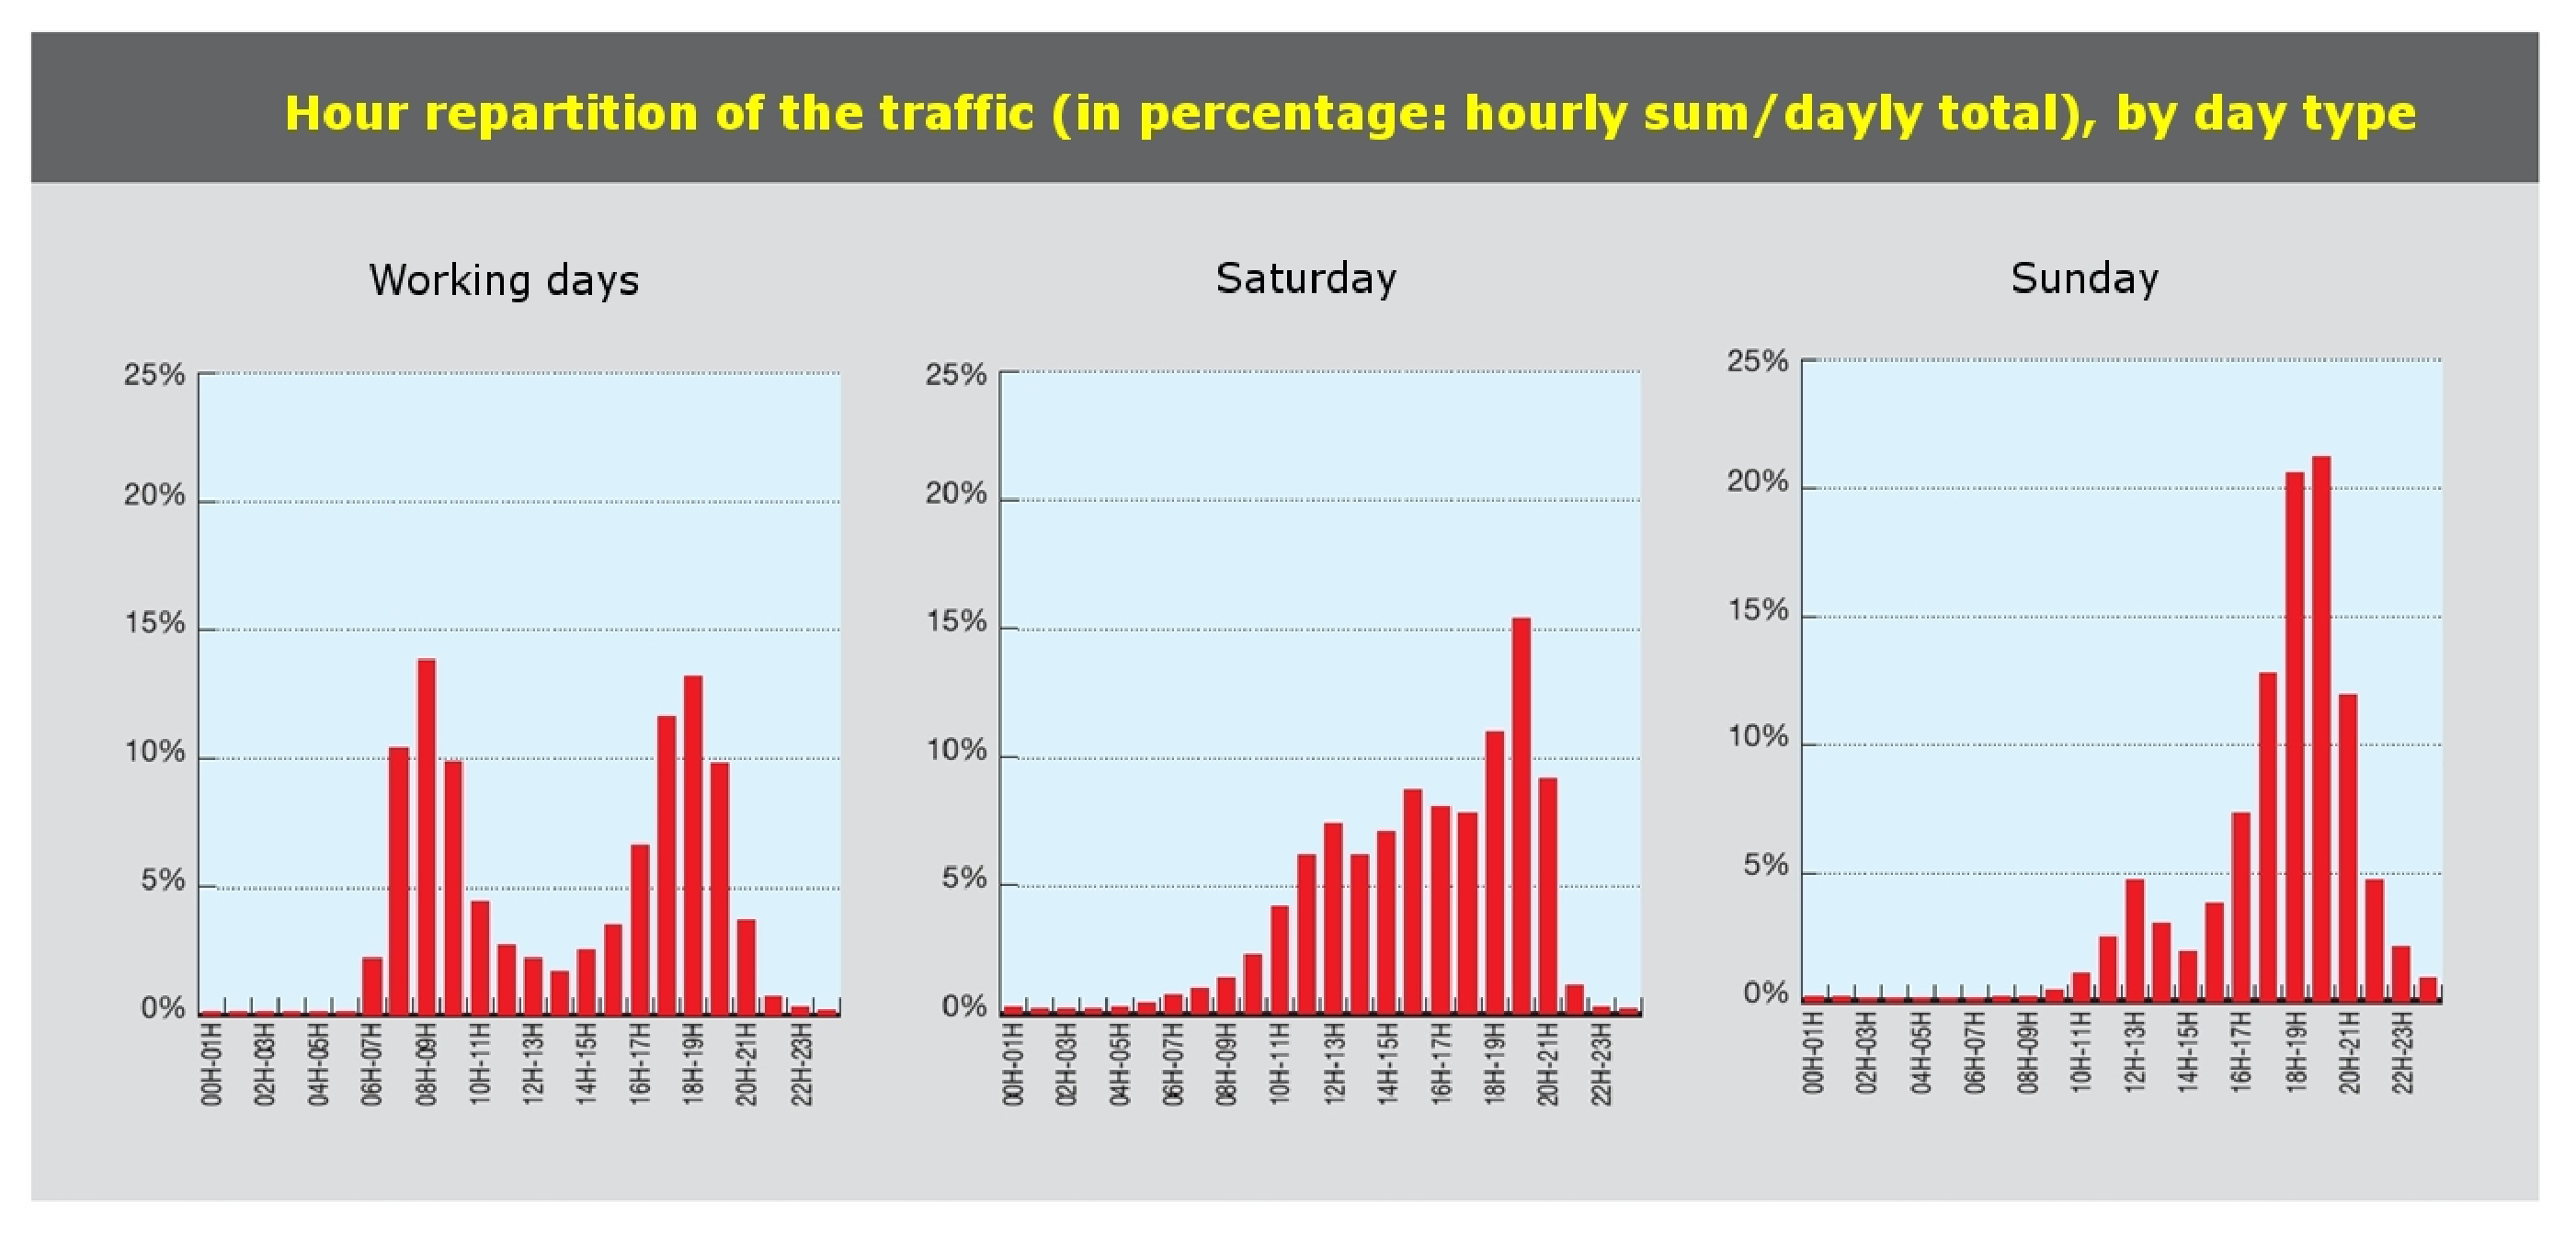
\includegraphics[width=8 cm,height=4.25 cm,angle=0]{traffic-repartition-by-day}
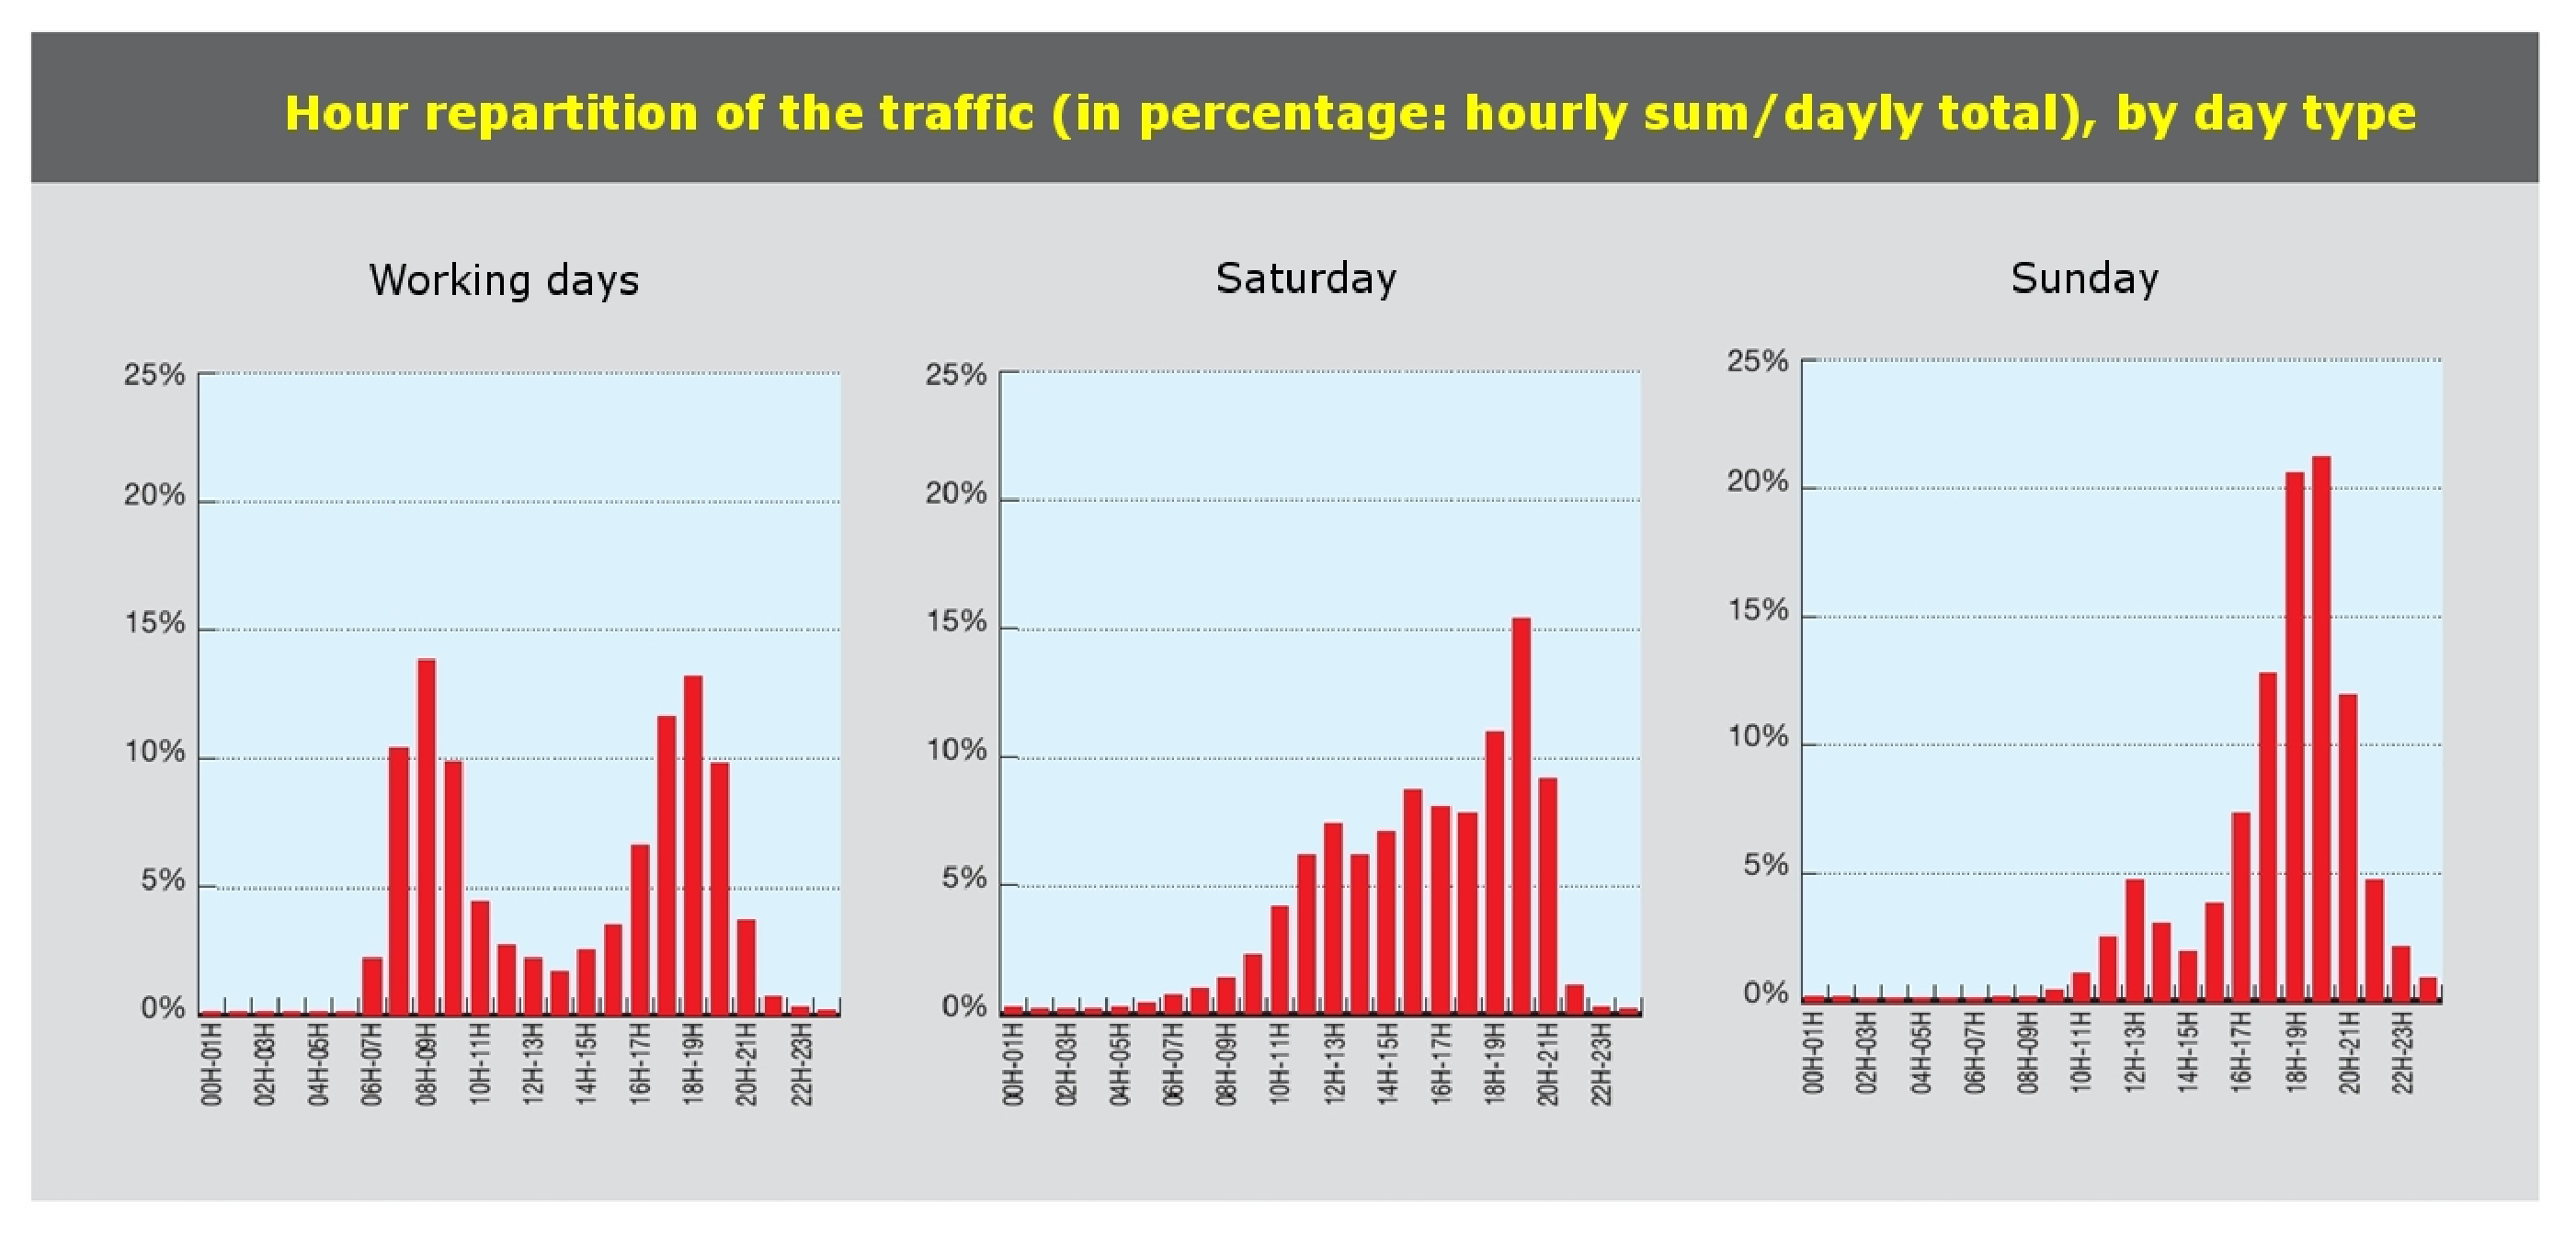
\includegraphics[width=.9\textwidth]{traffic-repartition-by-day}
\end{center}
\vskip -0.5cm
\caption{Traffic Repartition by Day and Hour Slices}
\label{figure-traffic-repartition-by-day}
\end{figure}

The evolution of the traffic can thus be approximated by a set of pre-computed reference traffic situations. 
For instance, on a week day, the evolution of the traffic can be characterized with 5 reference traffic situations  (cf. figure \ref{figure-traffic-situation}). We consider three intervals of values for the global indicator and distinguish between morning (S$_1$, S$_2$) and evening travels (S$_3$, S$_4$). 

\begin{figure}[h!]
\begin{center}
%\vskip -0.3cm
%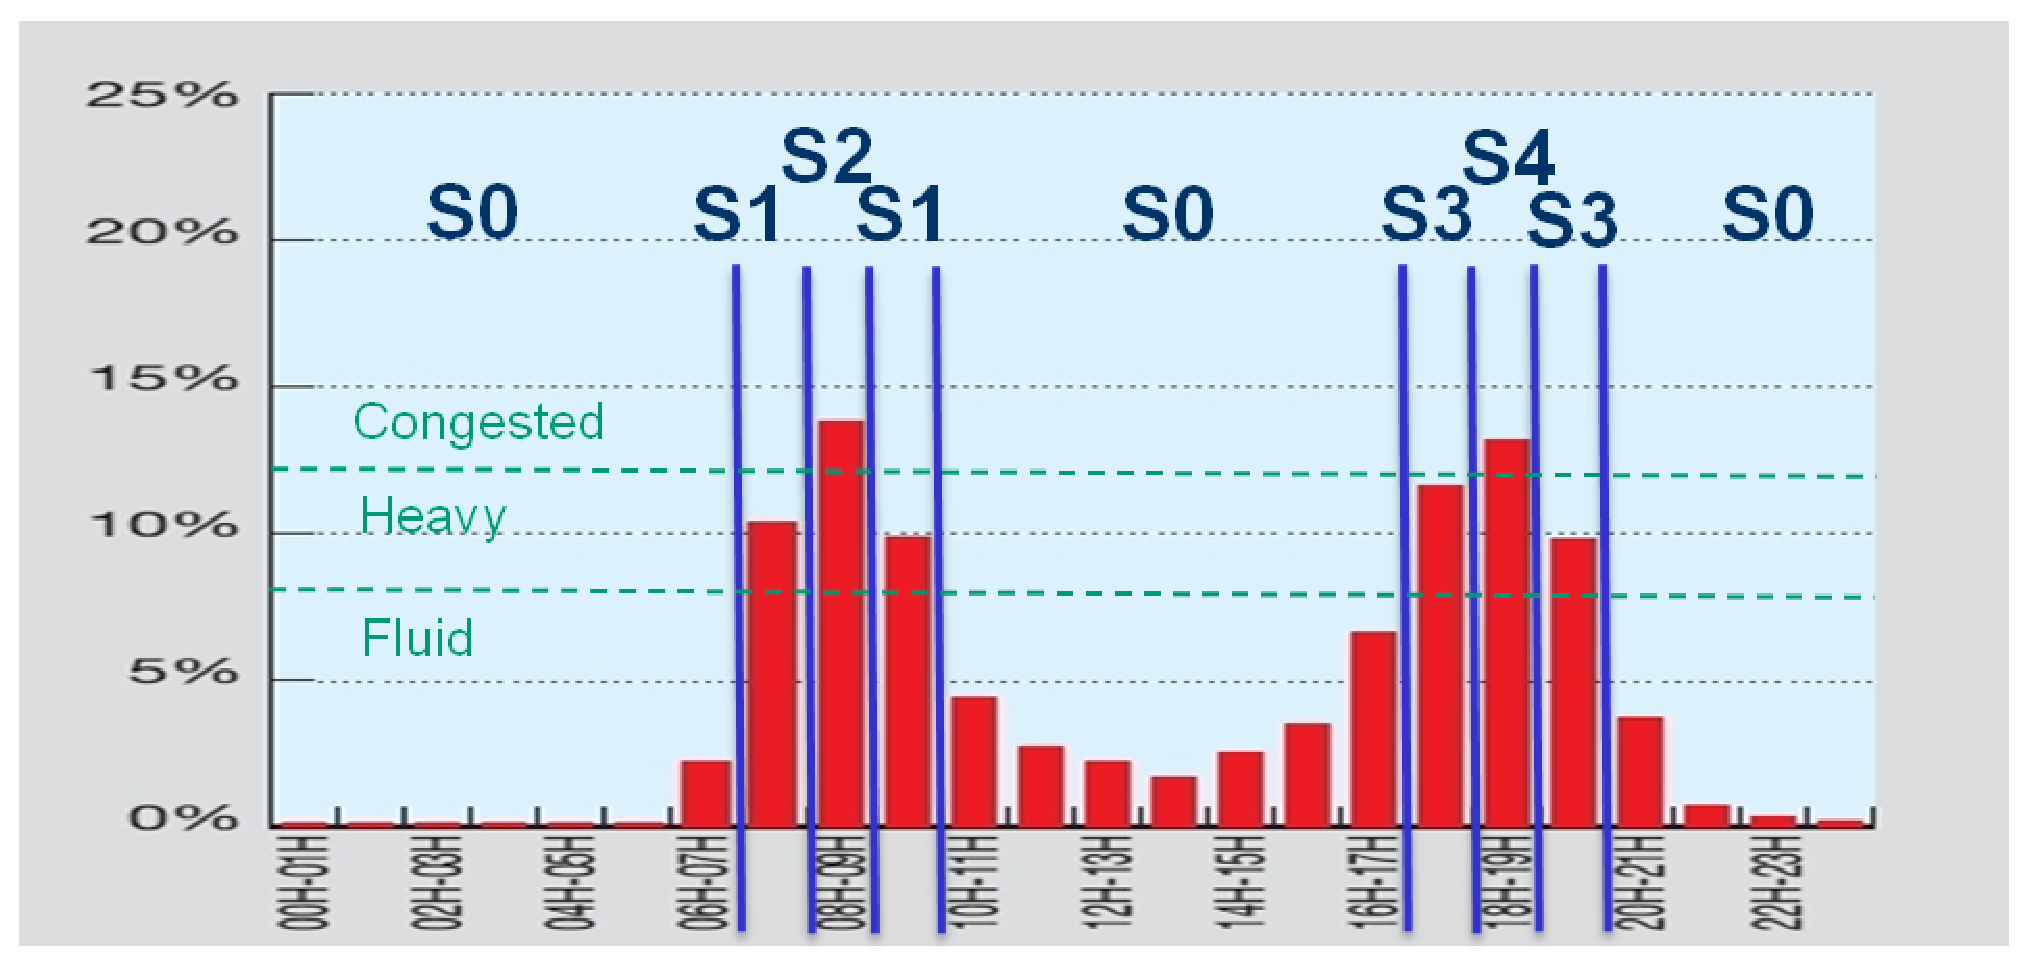
\includegraphics[width=8 cm,height=4.25 cm,angle=0]{traffic-situation}
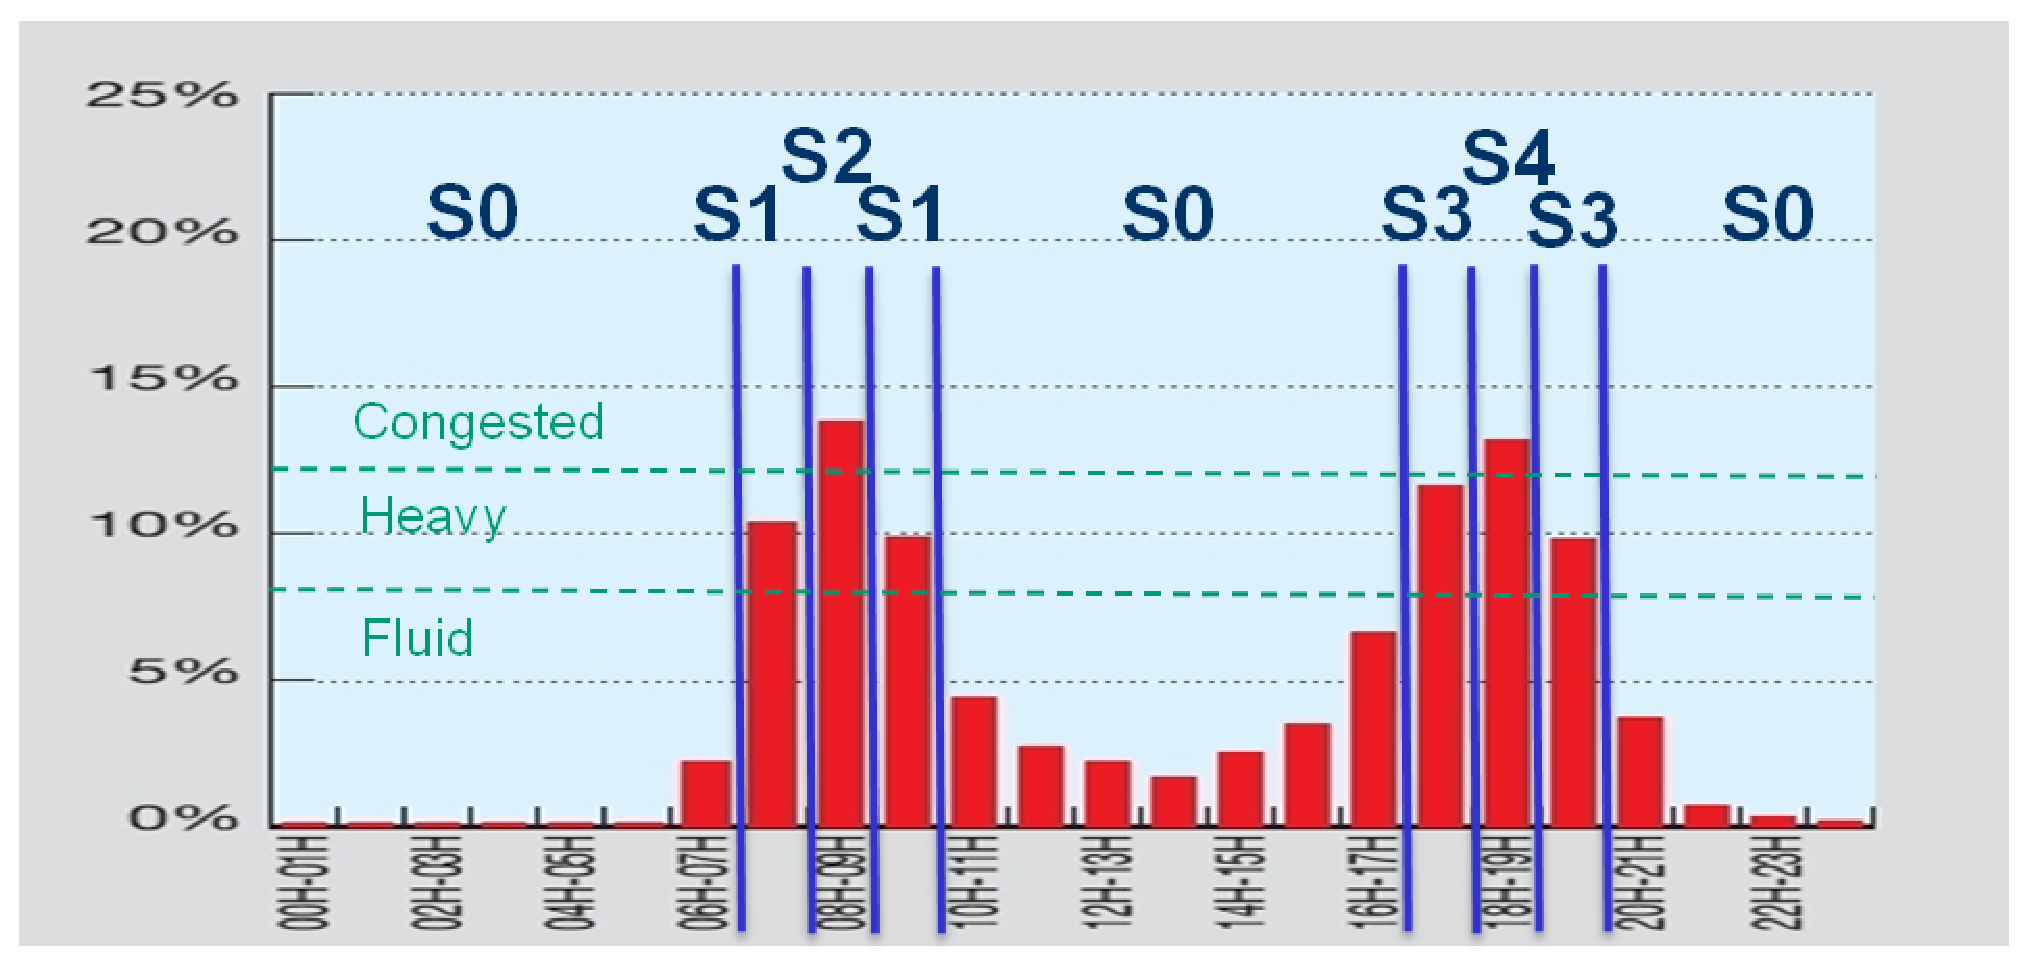
\includegraphics[width=.9\textwidth]{traffic-situation}
\end{center}
%\vskip -0.5cm
\caption{Traffic Reference Situations}
\label{figure-traffic-situation}
\end{figure} 

A prediction of the traffic evolution can then be defined as a temporal sequence of situations chosen among this reference set: S$_0$, S$_1$, S$_2$, S$_1$, S$_0$, S$_3$, S$_4$, S$_3$, S$_0$.  The resulting prediction model is then reduced to the set of travel time estimates between any two points of the network for a given reference situation. These travel times can be produced by any external traffic forecaster (macroscopic or statistical) and stored in abacuses for different traffic situations. The traffic prediction is then simply obtained from these abacuses and the sequence of reference situations. More accuracy is gained by increasing the number of reference situations or intermediate points.

Using this transit time prediction model, we can now take into account the evolution of the traffic on the rescue operations as well as the impact of police blocking actions on selected roads.

\chapter{Timed Initial Literals in CPT}
% D�finition, syntax, state-of-the-art, few words on the impact on implementation in optimal CPT quite natural with constraint programming ...

We made the choice to use an optimal planner to assist in the definition of the emergency domain, in order to verify step-by-step that solving problems in this
domain yields well the best solutions we have in mind. Of course, optimal planners do not scale well in comparison to the best satisficing planners, which
would be a preferable choice in a production context; but this proved to be useful in a design context.

The emergency domain requires concurrency and actions with duration, so we used the CPT planner \cite{Vidal2006} which is still, as far as we know, the most 
efficient domain-independent optimal temporal planner. It must be noted that CPT does not compute plans in the full PDDL2.1 semantics \cite{foxlong2003} where
preconditions may be required at the beginning, at the end, or over the interval between these time points, and effects may happen either at the beginning or at
the end of an action. It rather computes plans in the \emph{conservative} semantics, where preconditions must be true at the beginning, effects are
produced at the end, and neither of them must be deleted by a concurrent action during the action execution. This de facto forbids plans with required
concurrency \cite{Cushing2007}, which is not needed in its full generality in our case, but simplifies the writing of the domain. Indeed, we only need
required concurrency to take into account the forecast of exogenous events (which happen concurrently with plan actions and may constrain them to
e.g. finish before some deadline), which is performed by using timed initial literals.

We extended CPT to handle timed initial literals in a very straightforward way.
Each timed initial literal of the form \texttt{(at <timepoint> <litteral>)}, meaning that the litteral $l$ must be true at the specified timepoint $t$ in
every plan, is translated into an action $a$ of duration 0 with no precondition and $l$ as effect. The insertion of such an action in every plan at the
specified timepoint is then forced in CPT by means of additional constraints: $InPlan(a)=true$ ($a$ belongs to every plan), and $T(a)=t$ ($a$ is executed at
timepoint $t$, and as its duration is 0, its effect $l$ is immediately made true). Finally, the mechanism described in \cite{Vidal2006} to introduce several
instances of the same action is disabled for the special actions introduced to handle timed initial literals.

\chapter{The Emergency Domain}

First of all, an urban area is defined as a set of locations such as the crisis zone, hospitals, police and fire stations which are connected by a PDDL table function giving an average transit time for several situations (free, heavy, congested) and several configurations of the road network (with open/closed roads). Since we can assume that the best route to connect any of these points for a given situation is known in advance (e.g. from an underground station to an hospital), useless path planning in the road network is avoided. Resources are mainly vehicles and equipment for casualty search, extraction, decontamination, triage, medical care and transportation, police units, and hospital beds. Hospitals have a limited capacity and are specialized so that the casualties are dispatched according to a bed type requirement.

% temporal planning

In order to capture an evolving environment according to some prediction we rely on PDDL2.2 timed initial literals.
To capture the traffic evolution we simply express the schedule of predicted traffic situations in the initial state. For instance:
\begin{center}
%\scriptsize
%%\spread
\begin{verbatim}
(:init
  (currentSituation heavy)
  (at 121 (not (currentSituation heavy)))
  (at 121 (currentSituation congested))
  (at 300 (not (currentSituation congested))))
\end{verbatim}
\end{center}

\noindent states that the traffic will be heavy in the time interval [0,120] and congested in [121, 300].
The average time to connect any two points with a vehicle is given in a PDDL function which defines an abacus for each traffic situation (free, heavy, or congested).
Hence to take the traffic situation into account, a {\tt move} action is written as follows:
\begin{center}
%\scriptsize
%\spread
\begin{verbatim}
(:durative-action move
 :parameters (?v - Vehicle ?p1 ?p2 - Place ?s - Situation)
 :duration (= ?duration (averageTime ?s ?p1 ?p2))
 :condition (and (currentSituation ?s)
                 (loc ?v ?p1))
 :effect (and (not (loc ?v ?p1)) (loc ?v ?p2)))
\end{verbatim}
\end{center}

In order to specify police operations which alter the traffic we have introduced street network configurations.
The nominal configuration is when all streets are clear. The other configurations correspond to all possible combinations of blocked streets (which are not so many since only main boulevards are concerned).
Abacuses are then extended in order to store transportation times within each possible configuration and each possible situation.
The {\tt move} action is then refined as follows:
\begin{center}
%\scriptsize
%\spread
\begin{verbatim}
(:durative-action move
 :parameters (?v - Vehicle ?p1 ?p2 - Place ?s - Situation
              ?c - Config)
 :duration (= ?duration (averageTime ?s ?c ?p1 ?p2))
 :condition (and (currentSituation ?s) (currentConfig ?c)
                 (loc ?v ?p1))
 :effect (and (not (loc ?v ?p1)) (loc ?v ?p2)))
\end{verbatim}
\end{center}
Police intervention on the road network is reflected in a {\tt switch} action devoted to switching between configurations:
\begin{center}
%\scriptsize
%\spread
\begin{verbatim}
(:action switchConfiguration
 :parameters (?c1 ?c2 - Configuration 
              ?v1 ?v2 - policeunit ?s - Situation)
 :duration (= ?duration (deployTime ?c1 ?c2 ?s))
 :condition (and (currentSituation ?s) (currentConfig ?c1)
                 (loc ?v1 ?s1) (loc ?v2 ?s2)
                 (available ?v2))
 :effect (and (not (available ?v2)) (available ?v1)
              (not (currentConfig ?c1))
              (currentConfig ?c2)))
\end{verbatim}
\end{center}
Two other {\tt switch} actions are specified for the cases where either the source configuration or the target one is the nominal network.
Another action describes how to secure the crisis zone and for which the number of police units involved is made proportional to the zone size.
Beside casualty extraction, decontamination, medical care, and triage, which are simple resource allocations, the dispatching of casualties is made dependent on the bed type required as defined by the open standard EDXL-HAVE \cite{oasis2009}: {\em AdultIntensiveCare}, {\em PediatricsIntensiveCare}, {\em MedicalSurgical}, {\em Burn}, {\em AdultPsychiatric}, {\em PediatricPsychiatric}, {\em NegativeFlowIsolation}, or {\em OperatingRooms}. A scenario is built up with a set of casualties with a bed type requirement chosen among the above categories and the dispatching is captured with the following action:

\begin{center}
%\scriptsize
%\spread
\begin{verbatim}
(:action host
 :parameters (?v - Victim ?h - Hospital ?n1 ?n2 - Natural
              ?b - BedType) 
 :condition (and (loc ?v ?h) (bedRequired ?v ?b)
                 (bedCapacity ?h ?b ?n1) (next ?n2 ?n1))
 :effect (and (not (bedCapacity ?h ?b ?n1))
              (bedCapacity ?h ?b ?n2)
              (not (loc ?v ?h))(rescued ?v)))
\end{verbatim}
\end{center}

The model is further refined to apply a priority to casualties who might die if they are not rescued before a temporal boundary. 
We add a {\em Coffin} bed type to the EDXL-HAVE list and a morgue in the scenario which is an hospital with such type of ``beds''. 
The morgue is artificially located very far from the crisis zone so that it is always better (i.e. faster) to have a casualty kept alive.
The evolving status of a casualty is expressed again with timed initial literals.

%For instance, the evolving status of victim2 from {\em AdultIntensiveCare} to {\em Coffin} after time 35, is simply expressed in the init state as follows:
%\begin{center}
%\scriptsize
%\begin{verbatim}
%(:init
%  (bedRequired victim2 AdultIntensiveCare)
%  (at 35 (not (bedRequired victim2 AdultIntensiveCare)))
%  (at 35 (bedRequired victim2 Coffin)))
%\end{verbatim}
%\end{center}
The following optimal solution plan was produced for a scenario involving 3 casualties:
\begin{center}
%\scriptsize
%\spread
\begin{verbatim}
0: (move truck_pma station9 crisis1 heavy c0) [14]
0: (move amb12 station9 crisis1 heavy c0) [14]
0: (move truck_rbc station10 crisis1 heavy c0) [16]
0: (move truck_ext station11 crisis1 heavy c0) [14]
0: (move amb22 station10 crisis1 heavy c0) [16]
0: (move pol1b station1 crisis1 heavy c0) [10]
0: (move amb31 station11 crisis1 heavy c0) [14]
10: (secureZone crisis1 medium pol1b) [2]
12: (moveToConfiguration c0 c1 pol1b crisis1 heavy) [3]
14: (installPMA truck_pma crisis1) [1]
14: (installExtraction truck_ext crisis1) [1]
15: (extract casualty3 truck_ext crisis1) [2]
15: (switchConfiguration c0 c1 pol1b heavy) [2]
16: (installDecontamination truck_rbc crisis1) [1]
17: (decontaminate casualty3 truck_rbc crisis1) [2]
17: (extract casualty2 truck_ext crisis1) [2]
19: (diagnose casualty3 truck_pma crisis1) [2]
19: (decontaminate casualty2 truck_rbc crisis1) [2]
19: (extract casualty1 truck_ext crisis1) [2]
21: (load casualty3 amb12 crisis1) [2]
21: (diagnose casualty2 truck_pma crisis1) [2]
21: (decontaminate casualty1 truck_rbc crisis1) [2]
23: (move amb12 crisis1 hop2 heavy c1) [10]
23: (load casualty2 amb22 crisis1) [2]
23: (diagnose casualty1 truck_pma crisis1) [2]
25: (move amb22 crisis1 hop1 heavy c1) [3]
25: (load casualty1 amb31 crisis1) [2]
27: (move amb31 crisis1 hop1 congested c1) [5]
28: (unload casualty2 amb22 hop1) [5]
32: (unload casualty1 amb31 hop1) [5]
33: (unload casualty3 amb12 hop2) [5]
33: (host casualty2 hop1 n4 n3 AdultIntensiveCare) [1]
37: (host casualty1 hop1 n3 n2 AdultIntensiveCare) [1]
38: (host casualty3 hop2 n2 n1 Burn) [1]
\end{verbatim}
\end{center}

In this solution plan, the first moves are under the configuration {\tt c0} and a {\tt heavy} traffic. At time {\tt 15}, the configuration is switched to {\tt c1} by police intervention, whereas at time {\tt 27} the traffic becomes {\tt congested}. {\tt casualty2} is also treated before {\tt casualty1} because he has a ``deadline'' at time {\tt 35}.


We have  run several scenarios of increasing  size with the last  release of CPT
extended to handle timed initial literals and get optimal solutions up to 10 casualties.
Another scenario includes a second attack occurring a few moment later which of course has an impact on the emergency planning.

\chapter{Multiobjectivization of the Emergency Domain}

Although time is of primary importance in an emergency context, other criteria might be of interest and obviously the cost is one of them.
Cost is directly related to the consumption of resources and is clearly antagonistic with time: with more resources we can go faster.
Since it would be difficult to know in advance what is the best trade-off between the two criteria for a given decision-maker and a given context, it is not possible to aggregate them with a weighted mean for instance.
Instead we will provide the set of non-dominated solutions, the so-called Pareto front which exhibits the best trade-offs.
The standard PDDL does not provide this capability but fortunately in this project we have been able to design and implement the Pareto multiobjective planner: \MODAE\ \cite{modae:ijcai2013}.

The experimentation campaign using \MODAE\ on this benchmark is described in the D6.3 deliverable.

For now let's have a look to the transformation.
First the global variable total-cost is defined to accumulate all costs invoke with the increase primitive.
As previously all costs are stored in abacuses which are called with dedicated functions.

In the following {\tt move} action, we simply add a cost of using a vehicle proportional to the traveled distance.

\begin{center}
%\scriptsize
\begin{verbatim}
(:action move
 :parameters (?v - Vehicle 
              ?p1 ?p2 - Place 
              ?s - SituationTraf
              ?i - Itineraire 
              ?c - TrafficConfig)
 :duration (= ?duration (tempsMoyen ?c ?s ?i ?p1 ?p2))
 :condition (and (currentSituationTrafForecasted ?s)
                 (currentTrafficConfig ?c)
                 (loc ?v ?p1))
 :effect (and (not (loc ?v ?p1))
              (loc ?v ?p2)
              (increase (total-cost) (coutVehicle ?p1 ?p2))))
\end{verbatim}
\end{center}

We add a {\tt move} action with the help of an helicopter which is much faster but of course much more expensive:

\begin{center}
%\scriptsize
\begin{verbatim}
(:action moveHelico
 :parameters (?v - Helico ?p1 ?p2 - Place)
 :duration (= ?duration (tempsHelico ?p1 ?p2))
 :condition (and (loc ?v ?p1))
 :effect (and (not (loc ?v ?p1))
              (loc ?v ?p2)
              (increase (total-cost) (coutHelico ?p1 ?p2))))
\end{verbatim}
\end{center}

We could of course integrate other costs but this is enough to make a proof of concept.


\chapter{Conclusion}

We have shown how to take into account a changing environment according to a given forecast and have highlighted it with traffic predictions in an urban crisis management scenario.
Since the solver is domain independent, the paradigm can be used for any environment change as soon as prediction is made possible.
Other types of crisis such as natural disasters or industrial accidents, as well as other types of forecast (e.g. the propagation of a contaminated cloud) might be addressed.

The combinatorial blow-up is obviously a bottleneck for an optimal temporal planner such as CPT and the next step will be to test the model with a satisficing planner.
On the application side the next gate will be the integration in a real life system.
Note that the tool can also be used to size the rescue forces or to support the design and updating of emergency protocols.


We have shown also how easy it is to introduce another criteria to qualify the solution plans and to provide a new benchmark for the brand new multiobjective planner \MODAE\ developed in WP3.

\chapter{References}


%\bibliographystyle{plain}
%\bibliography{icaps10}

\begin{thebibliography}{}
%\bibliographystyle{aaai}
\bibliographystyle{plain}

%\bibitem[\protect\citeauthoryear{Descartes}{2008}]{Descartes2008}
%DESCARTES - POLE SYSTEM@TIC � PARIS REGION Proposition de projet de coop{\'e}ration Version 1.2.1.

\bibitem{oasis2009}
Emergency Data Exchange Language (EDXL) Hospital AVailability Exchange (HAVE), V1.0.
\newblock OASIS Standard, 22 December 2009.

%\bibitem[\protect\citeauthoryear{Sytadin}{2010}]{Sytadin2010}
%www.sytadin.fr.

\bibitem{SytadinDayHourRepartition2004}
Les d\'eplacements sur le r\'eseau de voies rapides urbaines d'\^Ile-de-France (Ann\'ee 2004).
\newblock Direction R\'egionale de l'\'Equipement.
%  Observation des d\'eplacements sur Voies Rapides.
%\newblock http://www.dir.ile-de-france.developpement-durable.gouv.fr/IMG/pdf/Deplacements\_VRU\_AN\_2004\_cle59612c.pdf
%\newblock http://www.dir.ile-de-france.developpement-durable.gouv.fr

%\bibitem[\protect\citeauthoryear{Sytadin}{2008}]{SytadinGeographicalRepartition2008}
%Les d\'eplacements sur le r\'eseau de voies rapides urbaines d�\^Ile-de-France.
%\newblock Direction R\'egionale de l'\'Equipement (DRE), Observation des d�placements sur Voies Rapides.
%%\newblock http://www.dir.ile-de-france.developpement-durable.gouv.fr/IMG/pdf/indicateurs\_2007\_2008\_cle6ff7a5.pdf
%\newblock http://www.dir.ile-de-france.developpement-durable.gouv.fr

\bibitem{Aligne2009}
Aligne, F.
\newblock Which Information and Decision Support System for the Crisis Management?
\newblock In NATO RTO Symposium, IST086, C3I for Crisis, Emergency and Consequence Management, 2009.

\bibitem{AligneSaveant2010}
Aligne, F.; and Sav\'eant, P.
\newblock Gestion de crise : optimisation de la mise en {\oe}uvre des plans de secours.
\newblock In Workshop Interdisciplinaire sur la S{\'e}curit{\'e} Globale ({\em WISG 2010}).

\bibitem{Barbulescu2010a}
Barbulescu, L.; Rubinstein, Z.B.; Smith, S.F.; Wilkins, D.E.; and Zimmerman, T.L.
\newblock Distributed Scheduling Agents for Disaster Response.
\newblock In ICAPS2010 Scheduling and Planning Applications woRKshop ({\em SPARK 2010}).

\bibitem{Barbulescu2010b}
Barbulescu, L.; Rubinstein, Z.B.; Smith, S.F.; and Zimmerman, T.L.
\newblock Distributed Coordination of Mobile Agent Teams: The Advantage of Planning Ahead.
\newblock In {\em $9^{th}$ International Conference on Autonomous Agents and Multiagent Systems (AAMAS 2010)}, pp. 10-14, 2010.

\bibitem{Castillo2006}
Castillo, L.; Fernandez-Olivares, J.; Garc{\'i}a-P{\'e}rez, {\'O}.; and Palao, F.
\newblock Efficiently Handling Temporal Knowledge in an HTN Planner.
\newblock In {\em $16^{th}$ International Conference on Automated Planning and Scheduling (ICAPS 2006)}, pp. 63-72, 2006.

%\bibitem[\protect\citeauthoryear{Cooper and Maris and Regnier}{2010}]{Cooper2010}
%Cooper, M.; Maris, F.; and R{\'e}gnier, P.
%\newblock Compilation of a High-Level Temporal Planning Language into PDDL 2.1.
%\newblock In {\em $22^{th}$ International Conference on Tools with Artificial Intelligence (ICTAI)}, 2010.

\bibitem{Cushing2007}
Cushing, W.; Kambhampati, S.; Mausam; and Weld, D.
\newblock When is Temporal Planning Really Temporal?
\newblock  In  {\em  $20^{th}$  International  Joint  Conference  on  Artificial
  Intelligence (IJCAI)}, pp. 1852-1859, 2007.

\bibitem{DanechPajouh2003}
Danech-Pajouh, M.
\newblock Les mod{\`e}les de pr{\'e}vision du dispositif Bison fut{\'e} et leur {\'e}volution.
\newblock Recherche Transports S{\'e}curit{\'e} RTS n.78, janvier-mars 2003.

\bibitem{Edelkamp2004}
Edelkamp, S.; and Hoffmann, J.
\newblock PDDL 2.2: The Language for the Classical Part of IPC-4. 
\newblock In Proceedings of the International Planning Competition. {\em $14^{th}$ International Conference on Automated Planning and Scheduling (ICAPS 2004)}, pp. 1-7, 2004.

\bibitem{Fdez-Olivares2006}
Fernandez-Olivares, J.; Castillo, L.; Garc{\'i}a-P{\'e}rez, {\'O}.; and Palao, F.
\newblock Bringing Users and Planning Technology Together. Experiences in SIADEX.
\newblock In {\em $16^{th}$ International Conference on Automated Planning and Scheduling (ICAPS 2006)}, pp. 11-20, 2006.

\bibitem{foxlong2003}
Fox, M.; and Long, D.
\newblock PDDL2.1: An Extension to PDDL for Expressing Temporal Planning Domains.
\newblock Journal of Artificial Intelligence Research, 20, pp. 61-124, 2003.

\bibitem{Haut2007}
Haut, B.
\newblock Modeling and Control of Road Traffic Networks.
\newblock Thesis, UCL. - ``FSA/INMA - D{\'e}partement d'ing{\'e}nierie math{\'e}matique'', 2007

\bibitem{modae:ijcai2013}
Khouadjia, M.~R., Schoenauer, M., Vidal, V., Dr\'{e}o, J., and Sav\'{e}ant, P.
\newblock {Pareto-Based Multiobjective AI Planning}.
\newblock In {\em 23$^{rd}$ International Joint Conference on Artificial
  Intelligence (IJCAI 2013)\/} (2013).

\bibitem{Lebacque2007}
Lebacque, J.-P.; Mammar, S.; and Haj-Salem, H.
\newblock Generic Second Order Traffic Flow Modeling.
\newblock In {\em $17^{th}$ International Symposium on Transporation and Traffic Theory (ISTTT)}, 2007.

\bibitem{Treiber2000}
Treiber, M.; Hennecke, A.; and Helbing, D.
\newblock Congested Traffic States in Empirical Observations and Microscopic Simulations.
\newblock Physical Review E, 62 (2), pp. 1805-1824, 2000.

\bibitem{Vidal2006}
Vidal, V.; and Geffner, H.
\newblock Branching and Pruning: An Optimal Temporal POCL Planner based on Constraint Programming
\newblock Artificial Intelligence, 170 (3), pp. 298-335.

%Ref traffic
%%%%%%%%%%%%%%%%
%Philippe L�g�, � S�curit� et s�ret� des transports - �tat de l�art �, Synth�se INRETS No 58, Contrat DRI/INRETS no 07 MTE048, Contrat DGITM/INRETS no 07 MTE048, Groupe op�rationnel no 2 du PREDIT, 2008

\end{thebibliography}


\end{document}